%% LyX 2.3.6.1 created this file.  For more info, see http://www.lyx.org/.
%% Do not edit unless you really know what you are doing.
\documentclass[american]{report}
\usepackage[T1]{fontenc}
\usepackage[latin9]{inputenc}
\setcounter{secnumdepth}{3}
\setcounter{tocdepth}{3}
\usepackage{xcolor}
\usepackage{graphicx}

\makeatletter
%%%%%%%%%%%%%%%%%%%%%%%%%%%%%% User specified LaTeX commands.
\usepackage{culmus}

\makeatother

\usepackage{babel}
\begin{document}
Qustion 4:

\textbf{The statement is False !}

Minimax is a recursive algorithm which is used to choose an optimal
move for a player assuming that the other player is also playing optimally.
Minimax generates the whole game tree, down to the leaves. 

Alpha beta pruning has no effect on minimax value computed for the
root.

But when we perform alpha-beta or minimax with resource limits i.e.
replacing the terminal utilitues with an evaluation function for non-terminal
positions the optimality is gone.

If we had a perfect heuristic we had to perform the search only one
move ahead, but in reality the evaluation functions are always imperfect.
Thus the algorithm is as good as it's evaluation function.

\textcolor{brown}{EXAMPLE HERE from Q1 !!! }

\pagebreak{}

Qustion 5:

suppose finet states: $s1,s2,s3,s4$

Define a utility function for the final states that doesn't define
a zero-sum game and according to which Minimax is optimal:

Recall: in zero-sum games $U(s,1)=-U(s,2)$ or $\sum_{k}^{N}U(s,k)=0$
sum of the utilities of all the playes is zero for all states.

for simplicity, let $U(s)=[U(s,1),U(s,2)]$.

For optimality we will assume that player 2 sicks to maximize his
utility.

a.

$U(s1)=[1,1]$

$U(s2)=[5,-3]$

$U(s3)=[0,0]$

$U(s4)=[1,-1]$

In the next example we can see that we defined a non zero sum game
and minimax return the optimal value (assuming player 2 is perfect).

The reason minimax is optimal in that example is because there is
a negative correlation between the two players i.e.

what is good for player 1 is bad for player 2. 

Player 1 can see that at the opponent move-in the worst scenario he
can get $[1,1]$ or $[0,0]$ for himself, and it's true because player's
2 best moves are going left in both cases (orange arrows).

So minimizing player's 1 utility in the opponnent move nodes was the
same as maximize opponent utilty and thus minimax is optimal in that
example.

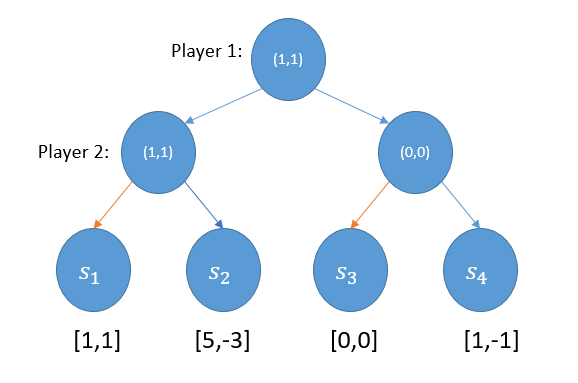
\includegraphics{Pics/5_a}

b.

Define a utility function according to which minimax isn't optimal. 

$U(s1)=[1,1]$

$U(s2)=[-1,-1]$

$U(s3)=[2,0.5]$

$U(s4)=[-1.5,0]$

In the below example we can see a case where minimax won't perform
the best moves. It's kind of cooperative game. 

Minimax trying to minimize it's own utility at the opponent nodes.
It will get's $[-1,-1]$ and $[-1.5,0]$ and chose to go left and
get minimax value of -1.

But the opponent in his turn will go left in his nodes (orange arrows).
Thus in the game Player 1 will get the utility of 1.

The best move for player 1 was to go right, because then the opponent
will take the lest node $[2,0.5]$ and player 1 utility could be 2.

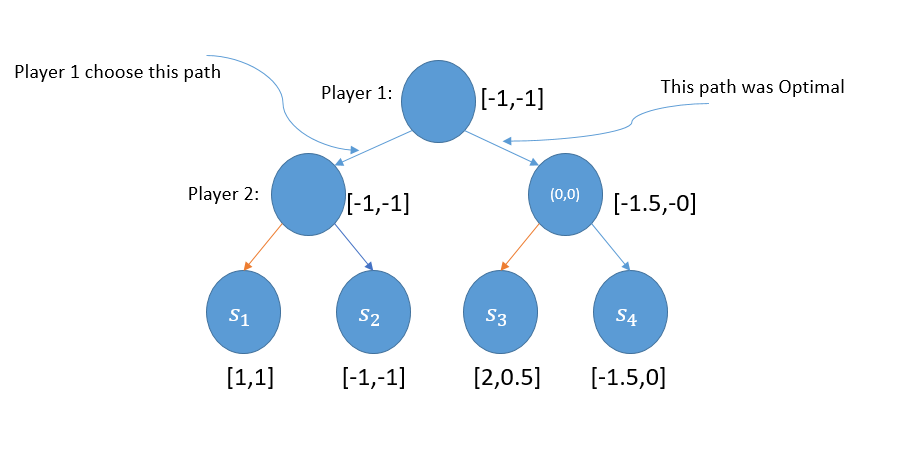
\includegraphics{Pics/7_c}

\textbf{Question 10:}

c.

An example for search space where SAHC dous not find an opttimal solition
with high probability is presented below.

Only if the initial starting point gets somewhere in the red interval
(along x-axis) it will climb to the global maximum, otherwise it 

will never reach the global maximum. If the initial starting point
will be somewhere along the purpule lines - SAHC will try to

maximize the value and reach a local maximum. So with high probability
SAHC will reach one of the ``sine'' peak.

In contrast, Simulated annealing algorithm can ``go down'' to find
a global peak, so along the purple lines this algoritm can go down
and

reach the peak with much higher probability thab SAHC.

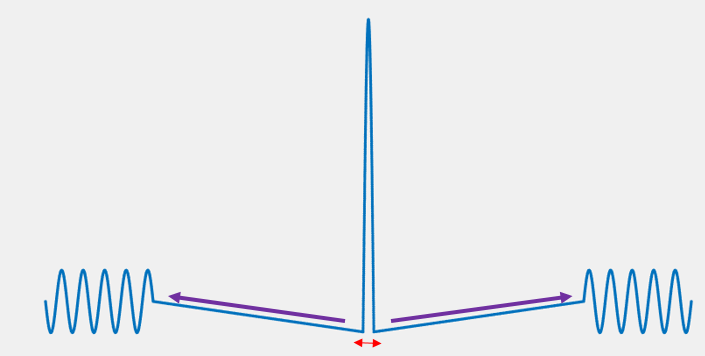
\includegraphics{Pics/7_c_2}
\end{document}
